\documentclass[a4paper,12pt]{article}

\usepackage{url}
\usepackage{epsfig}
\usepackage{graphics}
\usepackage{fancyhdr}
\usepackage{amsmath}
\usepackage{array,xcolor,colortbl}
\usepackage{multirow}
\usepackage{multicol}
\usepackage{float}
\usepackage{adjustbox}
\usepackage{enumitem}
\usepackage{caption}
\usepackage{subcaption}
\usepackage{tablefootnote}


\graphicspath{{pictures/}}

\title{Report Assignment 2 DD2380}
\author{\hspace*{-0.5cm}
GROUP 4:3\\
\begin{tabular}{cccc}
Vilmer Jonsson & Tor Strimbold\\
2001-06-26 & 1999-10-06 \\ 
vilmerj@kth.se & torstri@kth.se \\
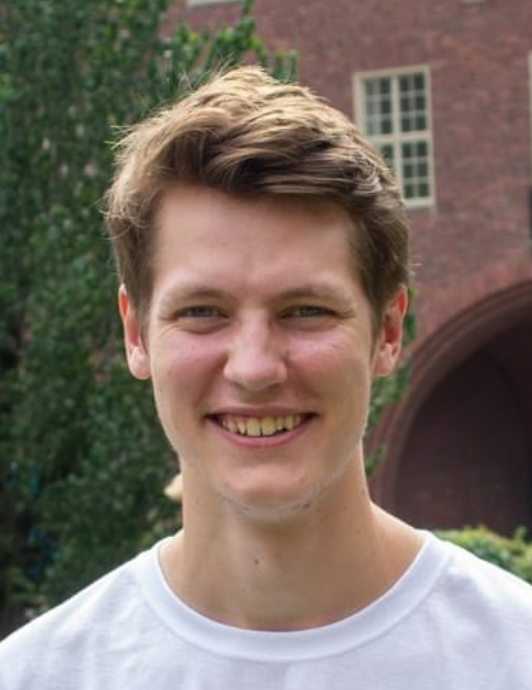
\includegraphics[width=0.13\linewidth]{Vilmer_Jonsson.jpg}
\end{tabular}} 
% Normally there will not be any pictures but we want
% these so that we can connect faces to names in the course
% We also want birthdates so that we can tell people with the same
% name apart
\date{\today}

\pagestyle{fancy}
\setlength{\headheight}{15pt}
\fancyhf{}
\lhead{DD2438} % DO NOT REMOVE!!!!
\rhead{Vilmer Jonsson \& Tor Strimbold} %% UPDATE WITH YOUR NAMES
\fancyfoot[C, CO]{\thepage}

\begin{document}

\maketitle
\thispagestyle{fancy}

\begin{abstract}



\end{abstract}


\clearpage

%%%%%%%%%%%%%%%%%%%%%%%%%%%%%%%%%%%%%%%%%%%%%%%%%%%%%%%%%%%%%
%%%%%%%%%%%%%%%%%%%%%%%%%%%%%%%%%%%%%%%%%%%%%%%%%%%%%%%%%%%%%
\section{Introduction}
\label{sec:intro}




\subsection{Contribution}

\subsection{Outline}


%%%%%%%%%%%%%%%%%%%%%%%%%%%%%%%%%%%%%%%%%%%%%%%%%%%%%%%%%%%%%
%%%%%%%%%%%%%%%%%%%%%%%%%%%%%%%%%%%%%%%%%%%%%%%%%%%%%%%%%%%%%
\newpage
\section{Related work}
\label{sec:relwork}
% \emph{Related Work section describing and referring to at least 5 research papers}

Example citation \cite{RussellNorvigAIBook3rd}.


%%%%%%%%%%%%%%%%%%%%%%%%%%%%%%%%%%%%%%%%%%%%%%%%%%%%%%%%%%%%%
%%%%%%%%%%%%%%%%%%%%%%%%%%%%%%%%%%%%%%%%%%%%%%%%%%%%%%%%%%%%%
\newpage
\section{Proposed method}
\label{sec:method}

The AI is implemented using the Monte Carlo Tree Search (MCTS) algorithm. The algorithm is divided into four main steps: selection, expansion, simulation, and backpropagation. Every turn, the algorithm is called and starts to run iteratively for a certain amount of time. 

Every node in the tree represents a state in the game. The root node is the current state of the game, and the children of the root node are the possible moves that can be made from the current state. A move is defined as all snakes in a team moving one step in a certain direction. If a move results in a collision, the move is invalid, and the node is not expanded. Thus, the number of children a node can vary, but is at most nine, since each snake can turn left or right, or go straight, and there are at most two snakes in a team. %% Detta är lite wonky

%% Vi kanske borde ha en figur här som visar hur trädet ser ut

\subsection{Selection}
In every iteration, there is a selection phase where the algorithm selects the best child node to explore. The selection starts from the root and then traverses down the tree, picking the best child at each level, until it reaches a leaf node, a node with no children.


The best child is selected based on the Upper Confidence Bound (UCB) formula. The formula is defined as:

\begin{equation}
    UCB = \text{score}_i + C \sqrt{\frac{\ln{N}}{n_i}}
\end{equation}

Where $\text{score}_i$ is the average score of the node, $N$ is the total times the parent node has been visited, $n_i$ is the number of times the node has been visited, and $C$ is a constant that controls the exploration-exploitation trade-off. The constant $C$ was set to $\sqrt{2}$ in this implementation, but no empirical testing was done to determine the optimal value. If the node has not been visited, the UCB value is set to infinity to ensure that the node is selected at least once if its parent node has been visited.


\subsection{Expansion}

The expansion phase is where the algorithm creates new child nodes for a leaf node. To create the child nodes, every possible move from the current state is 



\subsection{Simulation and Evaluation}




\subsection{Edge Cases}



\subsubsection{Head-To-Head Collisions}






%%%%%%%%%%%%%%%%%%%%%%%%%%%%%%%%%%%%%%%%%%%%%%%%%%%%%%%%%%%%%
%%%%%%%%%%%%%%%%%%%%%%%%%%%%%%%%%%%%%%%%%%%%%%%%%%%%%%%%%%%%%
\newpage
\section{Experimental results}
\label{sec:exps}



\subsection{Analysis of Outcome}



%%%%%%%%%%%%%%%%%%%%%%%%%%%%%%%%%%%%%%%%%%%%%%%%%%%%%%%%%%%%%
%%%%%%%%%%%%%%%%%%%%%%%%%%%%%%%%%%%%%%%%%%%%%%%%%%%%%%%%%%%%%
\newpage
\section{Summary and Conclusions}
\label{sec:summary}



%%%%%%%%%%%%%%%%%%%%%%%%%%%%%%%%%%%%%%%%%%%%%%%%%%%%%%%%%%%%%
%%%%%%%%%%%%%%%%%%%%%%%%%%%%%%%%%%%%%%%%%%%%%%%%%%%%%%%%%%%%%
\clearpage
\bibliographystyle{plain}
\bibliography{reflist}


\end{document}
